\documentclass{article}
\usepackage{kotex}
\usepackage{bm}
\usepackage{amssymb}
\usepackage{amsmath}
\usepackage{setspace}
\usepackage{graphicx}
\usepackage{booktabs}
\usepackage{subfigure}
\usepackage{url}

\begin{document}
\setstretch{1.4}

\title{페이저를 이용한 대역 필터의 주파수 응답 탐구}
\author{18009 고도형}
\maketitle

\section{페이저}

푸리에 분석은 어떠한 주기함수라도 서로 다른 여러 개의 정현파를 중첩하여 표현할 수 있음을 보장한다. 즉, 각기 다른 주파수와 진폭을 지닌 사인함수와 코사인함수를 일괄적으로 코사인함수로 환원하여 분석할 수 있다. 원운동의 정사영으로서 전류와 전압을 정현파의 형태로 기술할 수 있으므로 다음과 같은 전하의 운동을 생각한다. 원점으로부터 $A$만큼 떨어진 전하가 초기 위상 $\phi$를 가지므로 각진동수 $\omega$에 대하여 시간 $t$에 따른 전류 $x(t)$는 다음과 같다.

\begin{equation}
    x(t)=A \cos(\omega t+\phi)
\end{equation}

삼각함수의 덧셈정리를 이용하여 다음과 같이 전개할 수 있다.

\begin{equation}
    x(t)=A \cos(\omega t+\phi)=A(\cos\omega t\cos\phi-\sin\phi\sin\omega t)
\end{equation}

즉, 위상 $\phi$에 따른 물체의 위치를 좌표 $(X, Y)$로 기술할 수 있다.

\begin{equation}
    (X, Y)=(A\cos\phi, A\sin\phi)
\end{equation}

좌표를 복소평면에 대입하면 원운동을 허수축의 회전으로 기술할 수 있으므로 편리하다. $X$축을 실수축으로, $Y$축을 허수축으로 설정하면 교류전류의 페이저는 아래와 같이 나타난다.

\begin{equation}
    (X, Y)=X+jY=A\cos\phi+jA\sin\phi
\end{equation}

오일러 공식을 사용하면 이 좌표를 복소수 지수로서 정의할 수 있다.

\begin{equation}
    Ae^{j\phi}=A\cos\phi+jA\sin\phi
\end{equation}

\subsection{페이저 변환}

정현파 형식(Sinusoidal waveform)와 페이저 형식(Phasor) 사이에는 식 (5)과 같은 관계가 있다. 이를 응용하면 정현파 신호 $v(t)=V_m \cos(\omega t+\phi_V)$를 다음과 같이 페이저 형식으로 변환할 수 있다.

\begin{equation}
    \boldsymbol{V}=V_m e^{j(\omega t+\phi_V)}=V_me^{j\phi_V}
\end{equation}

이 $\boldsymbol{V}$를 교류전원장치의 전압의 페이저 형식이라 한다. 반대로, 페이저 형식을 알 때 이를 정현파로 바꿀 수 있다.

\begin{equation}
    \boldsymbol{V}=V_m e^{j(\omega t+\phi_V)}=V_m(\cos\omega t\cos\phi+\sin\phi\sin\omega t)=V_m \cos(\omega t+\phi_V)
\end{equation}


\section{전자소자의 페이저 표기}
전기 회로를 이루는 저항, 축전기, 그리고 유도기의 작용을 다음과 같이 페이저로 재정의할 수 있다.

\subsection{저항}
회로에 흐르는 교류전압과 교류전류에 대해 임의의 위상 $\phi_V$, $\phi_I$를 가정한다. 옴의 법칙(Ohm's Law)로 나타나는 특성방정식 $V=IR$을 적용하면 식(6)의 형식을 빌려 다음과 같이 나타낼 수 있다.

\begin{equation}
    V_me^{j\phi_V}=RI_me^{j\phi_I}
\end{equation}

실수부와 허수부의 값을 각각 비교하면 다음을 얻는다.

\begin{equation}
    V_m=I_mR
\end{equation}

이는 옴의 법칙과 동일하며 페이저 형식으로 나타내어진 회로에서도 저항은 동일하게 성립함을 확인할 수 있다.

\subsection{축전기}
특성방정식 $Q=CV$를 적용하고 전하와 전류의 관계로부터 식을 다음과 같이 변형한다.

\begin{equation}
    \frac{dq}{dt}=i=C\frac{dV}{dt}
\end{equation}

페이저 형식을 대입하여 정리하면 다음과 같다.

\begin{equation}
    V_m=\frac{I_m}{j\omega C}
\end{equation}

교류 회로에서는 축전기가 전하의 흐름을 방해하므로 이로부터 용량 리액턴스 $X_C=\frac{1}{j\omega C}$를 정의한다. 용량 리액턴스는 전류의 각진동수에 반비례하므로 높은 진동수를 가지는 고주파 전류일수록 값이 작다. 즉, 고주파 전류를 잘 통과시키는 반면, 저주파나 직류 전류는 통과시키지 않음을 알 수 있다.


\subsection{유도기}
특성방정식 $V=L\frac{di}{dt}$를 적용한다. 페이저 형식을 대입하여 정리하면 다음과 같다.

\begin{equation}
    V_m=j\omega LI_m
\end{equation}

교류 회로에서는 유도기가 전하의 흐름을 방해하므로 이로부터 유도 리액턴스 $X_L=j\omega L$를 정의한다. 유도 리액턴스는 전류의 각진동수에 비례하므로 높은 진동수를 가진 고주파 전류일수록 값이 크다. 즉, 상대적으로 저주파 전류나 직류를 통과시킨다.

\section{필터}
일반적으로 필터는 주파수 영역 중 원하지 않는 성분을 거르거나 원하는 성분만을 추출해 내기 위해 사용되는 회로를 일컫는다. 저항, 축전기, 유도기만을 사용하여 구성된 회로를 수동형 필터회로라 한다. 속도, 온도, 가속도, 힘, 소리 등 다양한 물리량을 계측한 데이터로부터 노이즈를 제거하기 위해 사용되는 필터 회로는 그 특성에 따라 저역통과필터, 고역통과필터, 대역통과필터, 그리고 대역저지필터의 4가지로 구분된다.

\subsection{저역통과필터}
저역통과필터(Low-Pass Filter; LPF)는 저주파 신호를 통과시키고 고주파 신호는 차단하는 필터로
유도기를 사용하여 구현할 수 있다.

\subsection{고역통과필터}


\section{주파수 응답}
어떠한 선형 회로 시스템에 대하여 시간에 따른 시스템의 입출력을 관측함으로서 회로를 구성하는 물리량의 변화를 관찰할 수 있다. 다음과 같은 형태의 선형 회로를 가정한다.

\begin{figure}[h]
    \centering
    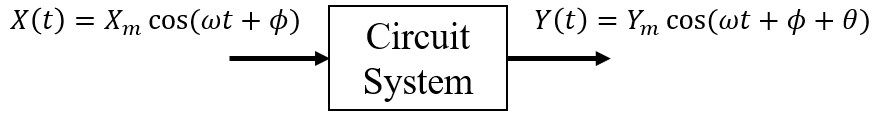
\includegraphics[scale=0.6]{./Linear Circuit System.png}
    \caption{Linear Circuit System}
\end{figure}

이제 두 회로의 입출력값을 관찰하여 기록하였더니 다음과 같았다고 하자.

\begin{figure}[h]
    \centering
    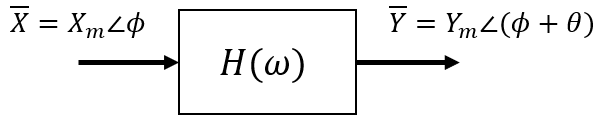
\includegraphics[scale=0.6]{./Frequency Response Function.png}
    \caption{Frequency Response Function}
\end{figure}

\section{시뮬레이션}

\section{결론}

\end{document}